
\documentclass[a4paper, 11pt, oneside]{Seminar}  % Use the "Seminar" style, based on the ECS Thesis style by Steve Gunn
\renewcommand{\familydefault}{\sfdefault} % Use sans-serif
\usepackage{helvet} % Helvetica font

\graphicspath{Figures/}  % Location of the graphics files (set up for graphics to be in PDF format)

% Include any extra LaTeX packages required
\usepackage[square, numbers, comma, sort&compress]{natbib}
\usepackage{verbatim} 
\usepackage{vector} 
\hypersetup{urlcolor=blue, colorlinks=true}
\usepackage{tikz} 
\usepackage[export]{adjustbox}
\usepackage{float}
\usepackage{lipsum}
\usepackage{todonotes}


\definecolor{shadecolor}{RGB}{180, 180, 180}

\hbadness=99999
\hfuzz=9999pt

\pagestyle{fancy}
\renewcommand\chaptermark[1]{\markboth{#1}{}}
\fancyhf{}
\fancyhead[L]{\emph\leftmark}
\fancyhead[R]{\thepage}

%% ----------------------------------------------------------------
\begin{document}
\frontmatter      % Begin Roman style (i, ii, iii, iv...) page numbering

\title  {Pure Synthetic Data Generation by the Example of a PostgreSQL and Python-based Tool}
\authors  {\href{mailto:Labian.Gashi@hsr.ch}{Labian Gashi}
}
\addresses  {\groupname\\\deptname\\\univname} 
\date       {Spring Semester 2020}


\maketitle

%% ----------------------------------------------------------------

\setstretch{1.2} 

\addtotoc{Abstract}  
\abstract{
	\addtocontents{toc}{\vspace{1em}}  
	Creation of realistic synthetic data is a challenging but important aspect of testing machine learning (ML) application and data science projects. The need for such data is constantly rising with the increase of the application of machine learning in different business functions.\\
\newline
There does not exist a lot of literature regarding synthetic data generation in the virtual world yet, the reason is that it is a pretty new concept for data engineers. This means that synthetic data generation is still in a "tabula rasa" state and the generation of such data can be done using many arbitrary approaches.\\
\newline
The idea or approach for this tool is creating a light-weight \href{https://en.wikipedia.org/wiki/Python_(programming_language)}{Python} application that collaborates with the \href{https://en.wikipedia.org/wiki/PostgreSQL}{PostgreSQL} database management system and uses real or realistic data contained in the PostgreSQL server in order to produce fully synthetic data. This generated data is not just anonymized data, but it rather advances even a step further by taking the shape and statistics of the real data and generating a set of data that has no direct association with the real data, but has the same or similar shape and feel of the real data.\\
\newline
The tool is very straight-forward to use and requires only the database connection parameters and the database containing the real data, every other function is done by the tool. It tries to simplify the process of generating synthetic data that can be used for testing maching learning applications or different data science projects. It is also easy and not cumbersome to set-up and has all the logic encapsulated within only a couple of scripts.\\
\newline
Keywords: \textit{synthetic data, artificial data, data anonymization, privacy, open data, data science, data engineering, open source, PostgreSQL, Python}
}

\clearpage  % Abstract ended, start a new page
%% ----------------------------------------------------------------

% The Acknowledgements page, for thanking everyone
\acknowledgements{
\addtocontents{toc}{\vspace{1em}}  % Add a gap in the Contents, for aesthetics

I would like to express my greatest gratitude towards my advisor \href{mailto:stefan.keller@hsr.ch}{Prof. Stefan Keller} for suggesting me this seminar to me and assisting me throughout the whole journey with his patient guidance and enthusiastic encouragement. \\
\newline
A huge thanks also goes to \href{mailto:johannes.wildermuth@hsr.ch}{Johannes Wildermuth} from the institute of HSR who helped me by supplying me with the first code scaffold for the tool. \\
\newline
Another special thanks goes to all the authors of the Python libraries and LateX templates that I used in order to complete this project. I would also like to send some appreciation to the GitLab team for having such a nice and neat application lifecycle tool for me to utilize. It provided me with a very comfortable code repository, CI/CD pipeline features and just generally a nice and consistent environment to have my application on.

}
\clearpage  % End of the Acknowledgements
%% ----------------------------------------------------------------


%% ----------------------------------------------------------------
\setcounter{tocdepth}{1}
\tableofcontents  % Write out the Table of Contents

%% ----------------------------------------------------------------
\mainmatter	  % Begin normal, numeric (1,2,3...) page numbering


\chapter{Introduction}
\section{General}
\lipsum[3-4]
\section{Goals \& Requirements}
\lipsum[9-11]
\section{Synthetic Data Generation}
\lipsum[8-10]
\section{Results}
\lipsum[5-6]

% Praxis part
\chapter{Overview of Synthetic Data Generation}
\section{Overview}
In more broad and accepted terms, synthetic data is "any production data applicable to a given situation that are not obtained by direct measurement" according to the McGraw-Hill Dictionary of Scientific and Technical Terms. \cite{McGrawSyntheticData}\\ Synthetic data is not only popular and useful in computer science but it is also important in other business functions/types such as: Healthcare Systems, Fraud Detection Systems etc. In this project, the data synthesization of various real-life data stored into databases is important. In this type of data synthesization, that data is initially analyzed and then transformed, or rather just used in order to generate another set of data, so it isn't really a transformation but rather just a mere "sample" or "pattern" for the synthesized data.\\
\newline
Various methods and techniques are used in order to synthesize data. The procedure of this examination, analysis and generation of the real data into synthetic data is explained thoroughly and in more detailed and technical terms in the \nameref{ch:technical_implementation} chapter.\\
Synthetic data does NOT refer to anonymized data, it is often a misconception or a "myth", there are various types of data transformations that can happen from real data such as: Anonymized data, artificial data, synthesized data etc. Moreover, there are also subtypes of the types mentioned above, which are of course, more detailed and technical.
\section{Data Synthesization}
Data synthesization is not a straight-forward process and it requires beforehand some sort of statistics and numbers that represent something. These statistics and numbers are then essential for the data synthesization process. The statistics must be correct and consistent so that the synthesization process can also be correct, with wrong statistics, we will get even worse results!\\
\newline
The statistics and numbers required for the synthesization are taken directly and only from the PostgreSQL database tables, especially from the \textit{pg\_stats} table. This table contains information such as: the most common values, what their frequencies are, the number of records that have NULL values, the histogram boundaries of the records, how distinct they are from one-another etc.\\
The \textit{pg\_stats} tables results, specifically, only the ones that the tool requires are first stored in a temporary dictionary and then read later in the data generation process. This information is transformed into Python objects and data types that are most convenient for the generation; manipulation done within this function is heavy. At the end of this function, objects with important and concise information are created, which are then used later for the actual generation/insertion of the data.\\
The synthesization process involves a lot of loops and arrays, and the data taken directly from the \textit{pg\_stats} table must be transformed into  information that is necessary for the further steps of the algorithm.
\newpage
\section{Data Generation}
Data generation somehow falls under the data synthesization process, it only is a little more specific and is used for process abstraction. It may fall under a separate category too, but these concepts are still a little bit unknown and not clearly-defined by the community. For this tool though, the data generation part falls under the data synthesization process.\\
\newline
After the information has been retrieved from the database (the statistics and numbers) and stored into the relative objects, the data generation part begins.\\
In this part, the data is generated in an iterative fashion and then later inserted directly into the secondary PostgreSQL empty database. Data generated here, must be consistent and in conformance with the databases schema. If something fails here (at a column), usually, the whole table is skipped completely because the generation cannot proceed for that table anymore.\\
The generation process reads through every information that has been created previously and generates data by relying on that information. Some sort of manipulation is done here too, the information created before serves only as a "guide" for generating the data, and it is not the actual data itself.\\
The tool iterates through each column of the table and checks the data type of that column (which was added before), and then based on the data type, it does some operations that generate the data, always of course, relying on the \textit{pg\_stats} statistics. If the table/column have no pg\_stats available, data is generated regardless, however, it is generated in a fully randomized fashion because there is no statistics or numbers to rely on.

\chapter{Implementation}
\label{ch:implementation}
\section{Overview}
The tool is a single lightweight Python script, executable from the shell terminal. The tool first connects to an existing PostgreSQL database (based on the passed arguments) and then based on whether \mintinline{bash}{-show} or \mintinline{bash}{-generate} arguments were passed, with \mintinline{bash}{-show} being the default one. The tool also accepts database connection parameters (all optional) such as \mintinline{bash}{-H, -P, -U} for connecting to the desired database server.\\
The \mintinline{bash}{-show} argument (which is the default one) will show the configuration of the database and the \mintinline{bash}{-generate} argument generates the synthesized data to the database with the name \mintinline{bash}{DBNAMEGEN}, which is one of the required arguments for this tool.\\
To be continued...
\section{Design and Implementation}
This tool is written and coded using the Python programming language.\\
It uses various Python libraries that are used for: argument parsing, various mathematical functions, making the connection to the PostgreSQL server easier etc.\\
It is a single python script that is to be executed using the shell terminal. It requires some arguments/parameters initially in order to evaluate the PostgreSQL server it needs to connect to, what database it relies on for generating the synthetic data and also the database where the synthetic data will be generated on.\\
To be continued...
\section{Tool Usage}
The tool is very straightforward to use. It contains a single Python script, with all the logic of connecting to the database and showing/generating the data in a single script. It is a script, designed to be executed from the terminal shell using the python command.\\
The tool is somehow split into two parts. The first part is the database connection part, which, based on the arguments given for the database and the PostgreSQL connection parameters, tries to connect to that database instance in the server. If everything there is successful, the tool then continues with the data synthesis part.\\
\newline
\textbf{Tool usage:} \newline
\mintinline{bash}{pgsynthdata [OPTIONS]... DBNAMEIN [DBNAMEGEN]} \\
\newline
\textbf{Tool options:}
\begin{itemize}
\item \mintinline{bash}{DBNAMEGEN} - Name of the database to be created
\item \mintinline{bash}{-show/--show} - Shows config (default)
\item \mintinline{bash}{-generate/--generate} - Generates new synthesized data to database \textit{DBNAMEGEN}
\item \mintinline{bash}{-O/--owner} - Owner of new database (default: same as user)
\item \mintinline{bash}{-v/--version} - Show version information, then quit
\item \mintinline{bash}{-h/--help} - Show tool help, then quit
\newline
\end{itemize}
\textbf{Connection options:}
\begin{itemize}
\item \mintinline{bash}{DBNAMEIN} - Name of the existing database to connect to
\item \mintinline{bash}{-H/--hostname} - Name of the PostgreSQL server (default: \textit{localhost})
\item \mintinline{bash}{-P/--port} - Port of the PostgreSQL server (default: \textit{5432})
\item \mintinline{bash}{-U/--user} - PostgreSQL server username
\newline
\end{itemize}
\textbf{Some usage examples:}
\begin{itemize}
	\item \mintinline{bash}{python pgsynthdata.py test postgres -show}
	\begin{itemize}
		\item Connects to database \textit{test}, host=\textit{localhost}, port=\textit{5432}, default user with password \textit{postgres}
		\item Shows statistics from certain tables in database \textit{test}
	\end{itemize}
	\item \mintinline{bash}{python pgsynthdata.py db pw1234 -H myHost -p 8070 -U testuser -show}
	\begin{itemize}
		\item Connects to database \textit{db}, host=\textit{myHost}, port=\textit{8070}, user=\textit{testuser} with password \textit{pw1234}
		\item Shows statistics from certain tables in database \textit{db}
	\end{itemize}
	\item \mintinline{bash}{python pgsynthdata.py dbin dbgen pw1234 -H myHost -p 8070 -U testuser -generate}
	\begin{itemize}
		\item Connects to database \textit{dbin}, host=\textit{myHost}, port=\textit{8070}, user=\textit{testuser} with password \textit{pw1234}
		\item Creates new database \textit{dbgen} with synthesized data
	\end{itemize}
	\item \mintinline{bash}{python pgsynthdata.py --version}
	\begin{itemize}
		\item Show the version of this tool and then quit
	\end{itemize}
\end{itemize}
It also uses all the other default PostgreSQL server settings when creating the new database such as: encoding, locale, collation, database template etc.
\begin{figure}[H]
	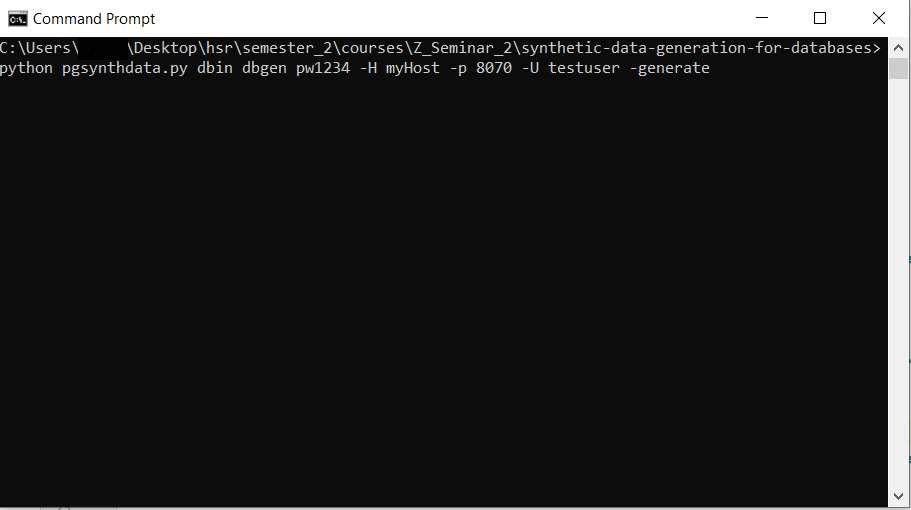
\includegraphics[width=\linewidth]{./Figures/Implementation/tool_example_cmd.png}
	\caption{Tool usage example}
\end{figure}

\chapter{Tool Evaluation}
\label{ch:tool_evaluation}
\section{Overview/Approach}
In this section, the approach for synthesizing and generating the data will be explained in a more technical fashion.\\
As explained before, the tool is executed via a single script, this script is connected to all of the other necessary python scripts which are all contained in the same directory (excluding the external libraries).
\subsection{Connecting to the Database}
The tool uses a library called \href{https://www.psycopg.org/}{psycopg}, which is a PostgreSQL adapter for the Python programming language. It provides a level of abstraction for doing various functions with the database server. It also provides us with different features such as: Exception handling, avoiding SQL-injections, thread-safe operations, large objects support etc. Some of the features described here were very important for this tool.\\
\newline
A set of the parameters that this tool takes are database connecting parameters like: database name, host name, TCP/IP port, postgres user and that users password. With the help of these parameters, the tool, using the psycopg library, connects to the desired database server. If this connection fails because of wrong credentials or the database not existing, a message is shown on the terminal explaining the reason why the connection failed and the program is exit. All of these operations and exception handlings are done with the help of this library.\\
\newpage
Example of a connection failure:
\begin{figure}[H]
	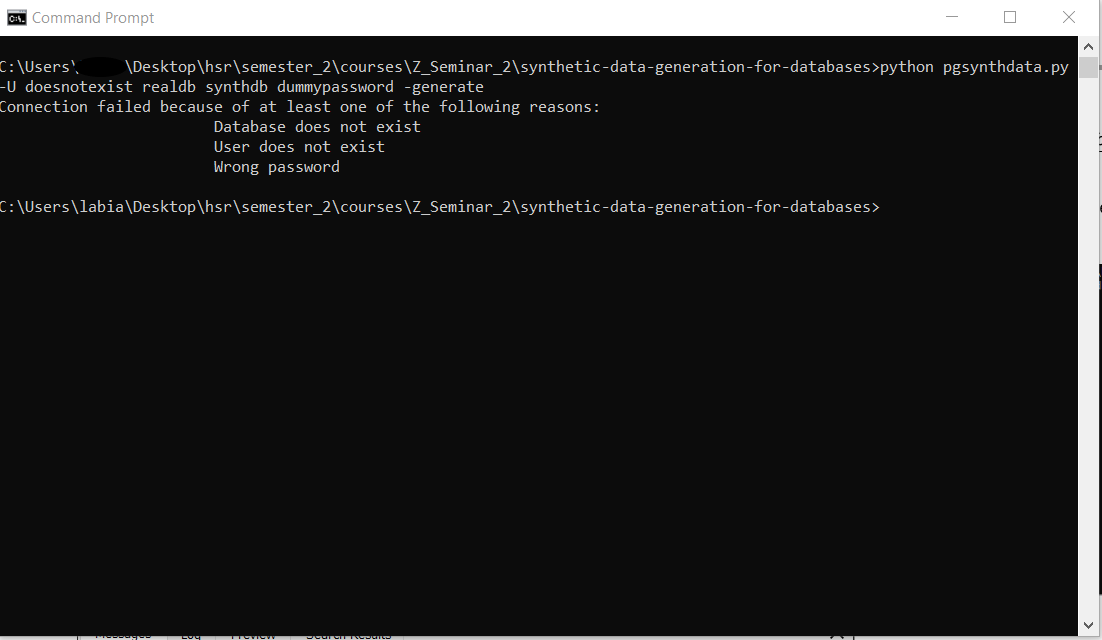
\includegraphics[width=\linewidth]{./Figures/ToolEvaluation/connection_failure_message.png}
	\caption{The message shown when the connection to the PostgreSQL database has failed}
\end{figure}
Depending on the parameters, whether \mintinline{bash}{-r} or \mintinline{bash}{--recreate} was passed, the tool either creates a new database, copying the complete schema of the primary database and leaving it empty, or it assumes that the database already exists and does not bother creating it and only connects to it.\\
The recreation is done using a combination of psycopg and shell commands that create a \textit{pg\_dump} file, specifying the connection parameters beforehand and dumping it into the same directory as the tool. After the database has been created, the \textit{pg\_dump} file is deleted from the machine because it is no longer needed.\\
\newpage
The function function that recreates the database:
\begin{minted}{python}
def copy_database_structure(args):
  print(f 'Copying the "{args.DBNAMEGEN}" database structure...')

try:
process = Popen(['pg_dump',
    '--dbname=postgresql://{}:{}@{}:{}/{}'.format(args.user,
      args.password,
      'localhost',
      '5432',
      args.DBNAMEIN),
    '-s',
    '-Fc',
    '-f', DUMP_FILE_PATH
  ],
  stdout = subprocess.PIPE)

process.communicate()[0]

process = Popen(['pg_restore',
    '--dbname=postgresql://{}:{}@{}:{}/{}'.format(args.user,
      args.password,
      'localhost',
      '5432',
      args.DBNAMEGEN),
    DUMP_FILE_PATH
  ],
  stdout = subprocess.PIPE
)

process.communicate()[0]
except Exception as error:
  sys.exit('Database structure could not be copied. Error: {}'.format(error))
finally:
if os.path.exists(DUMP_FILE_PATH):
  os.remove(DUMP_FILE_PATH)
\end{minted}
After the connection has been achieved and the database has been created/connected to, the tool proceeds with the data synthesization and generation part.\\
\subsection{Data Synthesization and Generation}
The data synthesization and generation part are the most crucial functions of this tool. They are the core logic of the tool and contain all the necessary methods for generating the synthetic data.\\
\newline
This logic of the tool is contained in a separate python script called \textit{data\_generator.py}, which contains the \textit{DataGenerator} class. This class contains all the necessary functions and attributes for generating the synthetic data.\\
It first connects to the primary database and loops through each table of the database (unless the \mintinline{bash}{-tables/--tables} parameter was supplied) and grabs information such as: primary keys, column information, pg\_stats for the table etc. It then stores this information into a huge nested dictionary, that is meant to hold such data (table names, primary keys, pg\_stats, column information). It fills only the important information and leaves the other information aside, creating a dictionary that contains only the necessary and vital statistics and numbers for the data generation.\\
\newline
After the dictionary has been fully supplied with the necessary information, another function named \textit{create\_insert\_query} is called. This function is a crucial function for the tool and it creates another sub-dictionary that contains the insert query for each table.\\
\newline
The algorithm steps for generating the data:
\begin{enumerate}
\item{Grab the important column information (data type, column name, numeric precision, numeric scale etc)}
\item{Grab information such as: the most common values and their frequencies, the average width of the column records, the factor of distinct values in the table.}
\item{Find out the number of distinct values that the tool should generate using the \textit{n\_distinct} pg\_stats value.}
\item{Since the default pg\_stats configuration stores only 100 records for the most common values and their frequencies, the numbers that their frequencies sum up to, usually does not reach 1 (unless the number of distinct values is less than 100), a dirichlet mathematical distribution is used to fill the leftover frequencies until the point that it reaches 1.\\
The Dirichlet distribution Dir(a) is a family of continuous multivariate probability distributions parameterized by a vector "a" of positive reals. It is a multivariate generalisation of the Beta distribution. Dirichlet distributions are commonly used as prior distributions in Bayesian statistics. \cite{WhatIsDirichletDistribution} \\
The dirichlet distribution is achieved in this tool with the help of the \href{https://numpy.org/}{NumPy} library.}
\item{Identify the columns data type and generate random data taken from an array of random values with weight that corresponds to the originalmost common frequencies of that column}
\item{Store all that data into a sub-dictionary that is used later for the final step of inserting the data into PostgreSQL}
\end{enumerate}
The figure below shows the probability density function for the Beta distribution with a number of alpha and beta values: \cite{DirichletDistributionSueLiu}
\begin{figure}[H]
	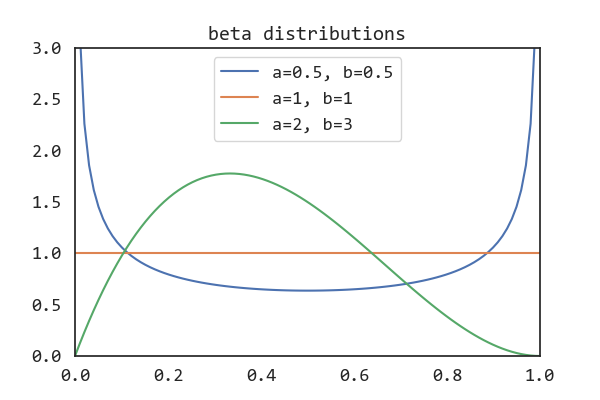
\includegraphics[width=\linewidth]{./Figures/ToolEvaluation/dirichlet_distribution.png}
	\caption{Probability density function for the Beta distribution (Dirichlet) \cite{DirichletDistributionSueLiu}}
\end{figure}
\newpage
\subsection{Data Insertion}
After the synthetic data has been generated, the tool loops through each table and inserts the synthetic data into the corresponding table using the psycopg library, logging any exception or important message to the user. If an exception is thrown while inserting the data into a specific table, the transaction is rolled back and the loop moves to the next table.\\
\newline
Data insertion function snippet:
\begin{minted}[breaklines]{python}
for table_name, insert_query in insert_dict.items():
  try:
    if insert_query:
      cursor.execute(
        sql.SQL(insert_query).format(
          table_name = sql.Identifier(table_name)
        )
      ) 
      connection.commit()
  except psycopg2.DatabaseError as db_error:
    sys.stdout.write(
      f 'An error occurred while inserting data into the "{table_name}" table. Error description: {db_error}.\n')
    connection.rollback()
\end{minted}
\section{Evaluation}
TBD...
\section{Results}
TBD...


%\lhead{\emph{Presentations}}
%\input{Chapters/Presentations}

\chapter{Conclusion}
\section{Discussion of the Results}
This tool was also presented in a webinar that has different attendees from different countries, many of them being members of the \href{https://www.swisspug.org/wiki/index.php/Swiss_PostgreSQL_Users_Group}{SwissPUG} group. The presentation was held online because of the COVID-19 restrictions but everything was made possible using screen-sharing.
The Swiss PostgreSQL Users Group (SwissPUG) is a group of people sharing an interest in promoting the usage of the open-source database system PostgreSQL. \cite{SwissPUGWiki} \\
\newline
The tool was presented and demonstrated using the Tennis\_ATP dataset, which can be found in the datasets appendix of \nameref{sec:tennis_atp_dataset}. The whole approach of synthesizing and generating the data was demonstrated, explaining everything along the demonstration being done and the reason why it's done in that fashion.\\
\newline
Future ideas and improvements were suggested by the attendees as well, some of them being:
\begin{itemize}
\item{\href{https://gitlab.com/labiangashi/pgsynthdata/-/issues/7}{Making use of extended statistics for inter-column correlations:}}
\item{\href{https://gitlab.com/labiangashi/pgsynthdata/-/issues/8}{Deducting the min/max from the pg statistics}}
\item{Synthesizing geographical data}
\item{Improving query plans by sharing the schema together with a set of test data with similar statistics (without revealing any confidential information) etc.}
\end{itemize}
Some of the attendees were interested in how the algorithm that synthesized the data worked in a more technical aspect, and some of the other attendees were already thinking of possible areas where they could apply this tool into.\\
\newline
Other ideas and nice to haves for the tool are:
\begin{itemize}
\item{\href{https://gitlab.com/labiangashi/pgsynthdata/-/issues/4}{Respect foreign key constraints}}
\item{\href{https://gitlab.com/labiangashi/pgsynthdata/-/issues/5}{Add configuration to add new functionality (incl. new data type generators or schema specific generators)}}
\item{\href{https://gitlab.com/labiangashi/pgsynthdata/-/issues/6}{Add support for data type geometry}}
\end{itemize}
\section{Achievements and Reflection}
The tool turned out to be a pretty interesting and light-weight tool, considering the work that it does. It can generate fully synthetic data with a single command and all it needs is one database consisting of real/realistic data, that's all.\\
\newline
Developing such a  tool was a very nice experience, the combination of Python, PostgreSQL, data science and data engineering resulted in this neat and light-weight tool that anyone can use to generate heaps amount of fully synthetic and realistic data. Synthetic data and artificial data were all relatively new terms for me in this seminar, I had heard about them before but never really knew the difference between them and their major usage. While developing this tool, all of these questions were answered to me. \\
\newline
The tool has a lot of space for improvements, such as adding new features or expanding the usage of current features. Some of these improvements are already logged in the \href{https://gitlab.com/labiangashi/pgsynthdata/-/issues}{GitLab repository}: \href{https://gitlab.com/labiangashi/pgsynthdata/-/issues}{https://gitlab.com/labiangashi/pgsynthdata/-/issues}
\section{Conclusion}
With this tool, mainly SW engineers but also other professionals can generate incredible amounts of data that they can use for testing their application, for training their machine learning models, for data science projects etc.\\
\newline
The neat thing about this tool is that it contains data that has no direct association with the real data (which means it is fully anonymized), it is merely generated data that has the same shape/size of the real data, but nothing concretely the same as the real data, hence the name fully synthesized data.\\
\newline
The tool is also very straight-forward to use and does everything itself, the most important factor before running the tool is having the primary database with realistic data and having another empty secondary database with the same schema, if that is not the case, the tool can also re-create the whole database, copying the schema of the primary database and having it ready for the tool to insert the data into. The amount of data that is generated can be optionally specified, if more data than the existing data in the primary database need to be generated. The larger the rows to generate, the more time it will take for the tool to complete its algorithm.\\
All the dependencies for running the tool are contained in a single text file called \textit{requirements.txt} and they can all be installed together in a single batch command before running the tool for the first time. The tool contains an open-source \href{https://opensource.org/licenses/MIT}{MIT License} and is open to improvements and new feature additions/suggestions.



%% ----------------------------------------------------------------
%\listoffigures  % Write out the List of Figures

%% ----------------------------------------------------------------
% Now begin the Appendices, including them as separate files

\addtocontents{toc}{\vspace{2em}} % Add a gap in the Contents, for aesthetics

\appendix % Cue to tell LaTeX that the following 'chapters' are Appendices

\lhead{\emph{Appendix}}
\chapter{Installation}

\chapter{Installation}
\section{Versions}
Used versions:
\begin{itemize}
	\item Lorem ipsum dolor sit amet, consectetuer adipiscing elit.
	\item Aliquam tincidunt mauris eu risus.
	\item Vestibulum auctor dapibus neque.
	\item Nunc dignissim risus id metus.
	\item Cras ornare tristique elit.
\end{itemize}

\section{Installing Docker}
To install docker, follow the instructions on \url{https://docs.docker.com/install/linux/docker-ce/debian/} or \url{https://docs.docker.com/install/linux/docker-ce/ubuntu/}.

\section{Installing Docker-Compose}
To install docker-compose, follow the instructions on \url{https://docs.docker.com/compose/install/}.

\section{Installing \& Configuring the Tool}
\lipsum[3]

\noindent\includegraphics[scale=0.5]{example-image-c} 
\chapter{Usage of Tool}
\label{a:tool_usage}
\textbf{Tool usage:} \newline
\mintinline{bash}{pgsynthdata [OPTIONS]... DBNAMEIN [DBNAMEGEN]} \\
\newline
\section{Options}
\textbf{Tool options:}
\begin{itemize}
	\item \mintinline{bash}{DBNAMEGEN} - Name of the database to be created
	\item \mintinline{bash}{-show/--show} - Shows database stats (default)
	\item \mintinline{bash}{-generate/--generate} - Generates new synthetic data to database \textit{DBNAMEGEN}
	\item \mintinline{bash}{-mf/--mf} - Multiplication factor for thegenerated synthetic data (default: 1.0)
	\item \mintinline{bash}{-tables/--tables} - Name(s) of table(s) to be filled, separated with ',', ignoring other tables (default: fill all tables)
	\item \mintinline{bash}{-r/--recreate} - (Re-)create new DBNAMEGEN and schema (default: don't recreate database/schema, just truncate the tables)
	\item \mintinline{bash}{-O/--owner} - Owner of new database (default: same as user)
	\item \mintinline{bash}{-v/--version} - Show version information, then quit
	\item \mintinline{bash}{-h/--help} - Show tool help, then quit
	\newline
\end{itemize}
\textbf{Connection options:}
\begin{itemize}
	\item \mintinline{bash}{DBNAMEIN} - Name of the existing database to connect to
	\item \mintinline{bash}{-H/--hostname} - Name of the PostgreSQL server (default: \textit{localhost})
	\item \mintinline{bash}{-P/--port} - Port of the PostgreSQL server (default: \textit{5432})
	\item \mintinline{bash}{-U/--user} - PostgreSQL server username
	\newline
\end{itemize}
\section{Usage Examples}
\textbf{Some usage examples:}
\begin{itemize}
	\item \mintinline{bash}{python pgsynthdata.py test postgres -show}
	\begin{itemize}
		\item Connects to database \textit{test}, host=\textit{localhost}, port=\textit{5432}, default user with password \textit{postgres}
		\item Shows statistics of the database \textit{test}
	\end{itemize}
	\item \mintinline{bash}{python pgsynthdata.py db pw1234 -H myHost -p 8070 -U testuser -show}
	\begin{itemize}
		\item Connects to database \textit{db}, host=\textit{myHost}, port=\textit{8070}, user=\textit{testuser} with password \textit{pw1234}
		\item Shows statistics of the database \textit{db}
	\end{itemize}
	\item \mintinline[breaklines]{bash}{python pgsynthdata.py dbin dbgen pw1234 -H myHost -U testuser -generate}
	\begin{itemize}
		\item Connects to database \textit{dbin}, host=\textit{myHost}, port=\textit{5432}, user=\textit{testuser} with password \textit{pw1234}
		\item Truncates tables of \textit{dbgen} and generates synthetic data into them
	\end{itemize}
	\item \mintinline{bash}{python pgsynthdata.py dbin dbgencreate pw123 -U myUser -generate -r}
	\begin{itemize}
		\item Connects to database \textit{dbin}, host=\textit{localhost}, port=\textit{5432}, user=\textit{myUser} with password \textit{pw123}
		\item Creates new database \textit{dbgencreate} with the same schema as \textit{dbin} and generates synthetic data into it
	\end{itemize}
	\item \mintinline[breaklines]{bash}{python pgsynthdata.py dbin dbgencreate pw123 -U myUser -generate -tables myTable1, myTable2}
	\begin{itemize}
		\item Connects to database \textit{dbin}, host=\textit{localhost}, port=\textit{5432}, user=\textit{myUser} with password \textit{pw123}
		\item Only truncates the \textit{myTable1} and \textit{myTable2} tables and generates synthetic into them
	\end{itemize}
	\item \mintinline{bash}{python pgsynthdata.py --version}
	\begin{itemize}
		\item Shows the version of this tool
	\end{itemize}
	\item \mintinline{bash}{python pgsynthdata.py --help}
	\begin{itemize}
		\item Shows the help information for this tool
	\end{itemize}
\end{itemize}
\chapter{Test Datasets}
For data synthesis, good and realistic data is necessary. For this project, many test datasets were used in order to implement, test and evaluate the tool. In this appendix, you will find some of the most important ones and some information/examples of them.
\section{Tennis ATP}
\label{sec:tennis_atp_dataset}
Tennis ATP is a dataset consisting of realistic data of the Tennis ATP (Association of Tennis Professionals). It includes rankings of players, data about the players themselves, data about the matches played between those players etc. \\
\newline
The repository for the complete data set can be found here: \url{https://github.com/JeffSackmann/tennis\_atp}. The complete dataset found in the repository however,  is not entirely used in this tool, only some chunks of it. The data set chunks used for this tool have been chosen and provided by my advisor: Prof. Stefan Keller.\\
\begin{figure}[H]
	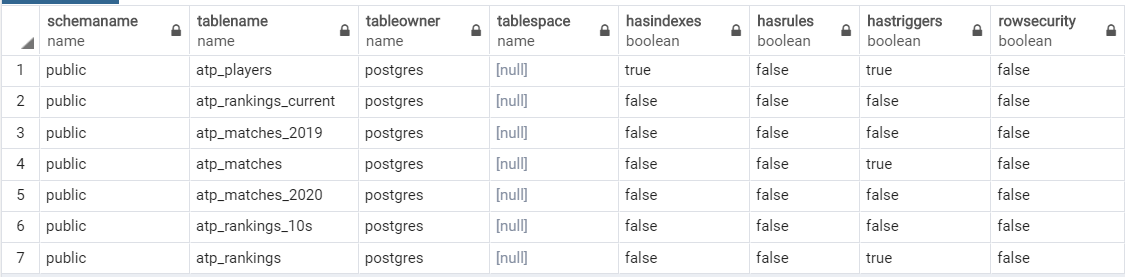
\includegraphics[width=\linewidth]{./Figures/Appendices/tennis_atp_schema.png}
	\caption{Tennis ATP database schema}
\end{figure}
\newpage
The columns of the tables are realistic and make sense. They also make sense in the context of synthesizing them.
\begin{figure}[H]
	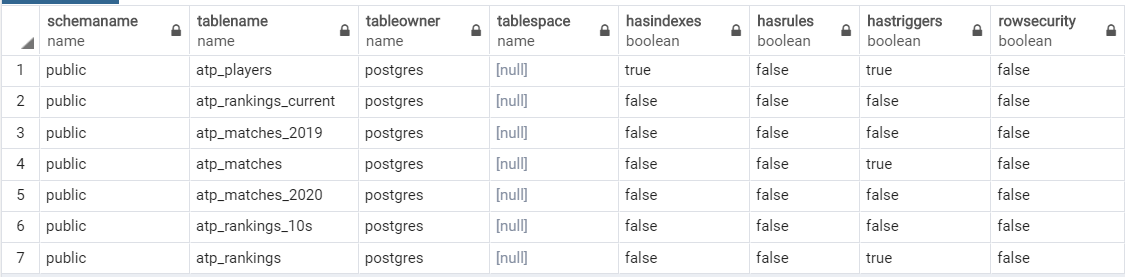
\includegraphics[width=\linewidth]{./Figures/Appendices/tennis_atp_schema.png}
	\caption{Tennis ATP database schema}
\end{figure}
\begin{figure}[H]
	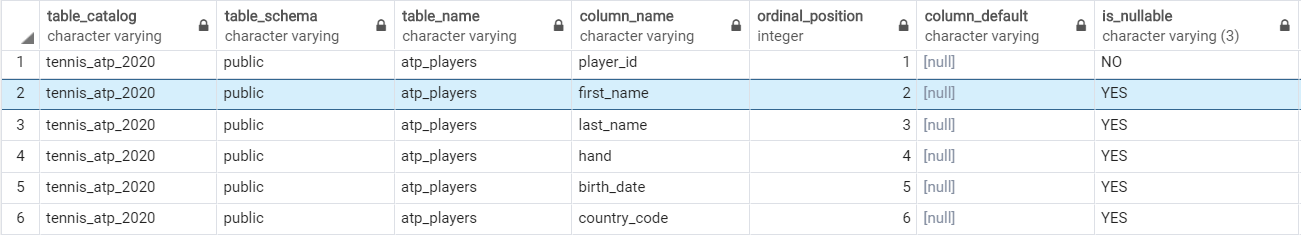
\includegraphics[width=\linewidth]{./Figures/Appendices/tennis_atp_players_schema.png}
	\caption{Tennis ATP "atp\_players" table schema}
\end{figure}
\begin{figure}[H]
	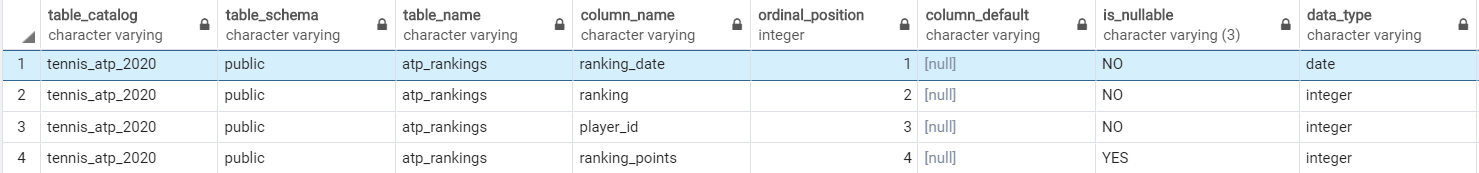
\includegraphics[width=\linewidth]{./Figures/Appendices/tennis_atp_rankings_schema.png}
	\caption{Tennis ATP "atp\_rankings" table schema}
\end{figure}
\begin{figure}[H]
	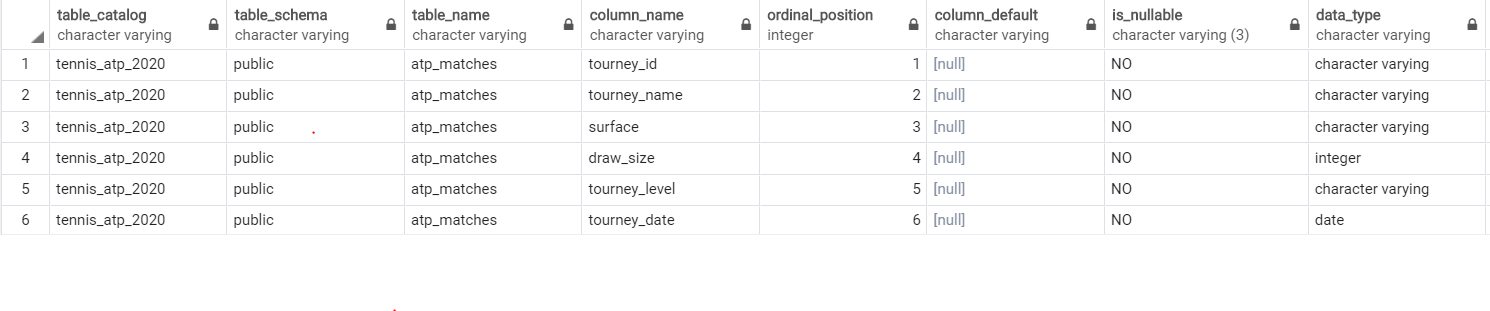
\includegraphics[width=\linewidth]{./Figures/Appendices/tennis_atp_matches_schema_1.png}
	\caption{Some information from the Tennis ATP "atp\_matches" table schema \#1}
\end{figure}
\begin{figure}[H]
	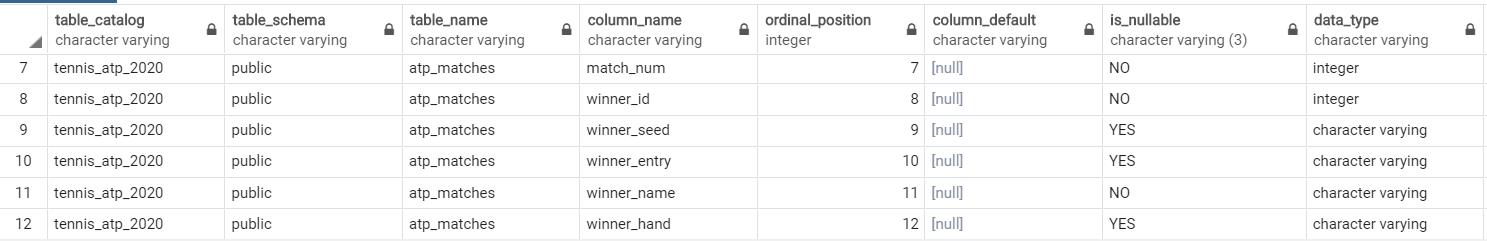
\includegraphics[width=\linewidth]{./Figures/Appendices/tennis_atp_matches_schema_2.png}
	\caption{Some information from the Tennis ATP "atp\_matches" table schema \#2}
\end{figure}
\section{IMDB}
\section{New York Taxi}

\newpage
\addtocontents{toc}{\vspace{2em}}  % Add a gap in the Contents, for aesthetics
\backmatter

%% ----------------------------------------------------------------
\label{Bibliography}
\lhead{\emph{Bibliography}}  % Change the left side page header to "Bibliography"
\bibliographystyle{unsrtnat}  % Use the "unsrtnat" BibTeX style for formatting the Bibliography
\bibliography{Bibliography}  % The references (bibliography) information are stored in the file named "Bibliography.bib"

\end{document}  % The End
%% ----------------------------------------------------------------